\PassOptionsToPackage{quiet}{xeCJK}
\documentclass[withoutpreface,bwprint]{cumcmthesis}


\usepackage{geometry}
\geometry{left=2.5cm, right=2.5cm, top=2.5cm, bottom=2.5cm}

% 中文字号调整
\renewcommand{\rmdefault}{ptm}  % Times New Roman
\zihao{-4}  % 四号
\renewcommand{\arraystretch}{1.4}

% 表格与排版
\usepackage{tabularx}
\usepackage{booktabs}  % 三线表
\usepackage{makecell}  % \Xhline
\usepackage{diagbox}   % 斜线表头
\newcolumntype{C}{>{\centering\arraybackslash}X}
\newcolumntype{R}{>{\raggedleft\arraybackslash}X}
\newcolumntype{L}{>{\raggedright\arraybackslash}X}
\usepackage{etoolbox}
\BeforeBeginEnvironment{tabular}{\zihao{-5}}

% 数学公式
\usepackage{amsmath,amssymb}

% 文献管理
\usepackage[numbers,sort&compress]{natbib}  

% 链接、图形
\usepackage{url}
\usepackage{subcaption}  

% TikZ 绘图
\usepackage{tikz}
\usetikzlibrary{calc, arrows.meta, positioning, shapes.geometric, fit, backgrounds, decorations.text}

% 框架
\usepackage[framemethod=TikZ]{mdframed}

% 自定义颜色与命令
\definecolor{mygray}{RGB}{208,208,208}
\definecolor{mymagenta}{RGB}{226,150,116}
\newcommand*{\mytextstyle}{\sffamily\Large\bfseries\color{black!85}}

\newcommand{\arcarrow}[3]{%
   \pgfmathsetmacro{\rin}{1.7}
   \pgfmathsetmacro{\rmid}{2.2}
   \pgfmathsetmacro{\rout}{2.7}
   \pgfmathsetmacro{\astart}{#1}
   \pgfmathsetmacro{\aend}{#2}
   \pgfmathsetmacro{\atip}{5}
   \fill[mygray, very thick] (\astart+\atip:\rin)
                         arc (\astart+\atip:\aend:\rin)
      -- (\aend-\atip:\rmid)
      -- (\aend:\rout)   arc (\aend:\astart+\atip:\rout)
      -- (\astart:\rmid) -- cycle;
   \path[
      decoration = {
         text along path,
         text = {|\mytextstyle|#3},
         text align = {align = center},
         raise = -1.0ex
      },
      decorate
   ](\astart+\atip:\rmid) arc (\astart+\atip:\aend+\atip:\rmid);
}

\tikzset{
  >={Latex[width=2mm,length=2mm]},
  base/.style = {rectangle, rounded corners, draw=black,
                 minimum width=4cm, minimum height=1cm,
                 text centered, font=\sffamily},
  startstop/.style = {base, fill=red!30},
  decision/.style = {diamond, draw, text centered, inner sep=0pt,
                     minimum width=4cm, minimum height=1cm, aspect=2,
                     font=\sffamily},
  process/.style = {base, minimum width=3.5cm, fill=orange!15,
                    font=\ttfamily},
}

% 文档基本信息
\title{生产过程中的决策问题}
\tihao{}
\baominghao{}
\schoolname{}
\membera{}
\memberb{}
\memberc{}
\supervisor{}
\yearinput{}
\monthinput{}



%%%%%%%%%%%%%%%%%%%%%%%%%%%%%%%%%%%%%%%%%%%%%%%%%%%%%%%%%%%%%
%% 正文
\begin{document}

\maketitle
\thispagestyle{empty}
\begin{abstract}



\textbf{对于问题一,}


   \keywords{} 

\end{abstract}
%%%%%%%%%%%%%%%%%%%%%%%%%%%%%%%%%%%%%%%%%%%%%%%%%%%%%%%%%%%%% 

% \tableofcontents  % 目录
% \newpage

%%%%%%%%%%%%%%%%%%%%%%%%%%%%%%%%%%%%%%%%%%%%%%%%%%%%%%%%%%%%%  
\pagenumbering{arabic}
\section{问题重述}

\subsection{问题背景}
为高效利用有效资源、减少生产成本、提高运营收益,优化生产决策是每个企业经营管理中的核心环节。某企业生产电子产品需采购两种零配件,并将其装配后形成成品,且成品合格性受零配件质量影响,因此企业需通过抽样检测控制零配件次品率,并对不合格成品选择报废或拆解。生产过程中需决策是否检测零配件或成品、是否拆解不合格品,并考虑调换市场退回品的损失。对此我们需要设计抽样方案、优化生产阶段决策,并推广到多工序多零配件场景,以通过成本与风险平衡提升整体效益。


\subsection{题设数据}
\textbf{表一}给出了两种零配件和成品的次品率,以及购买单价、检测成本、市场售价等参数信息。

\textbf{表二}给出了八个零配件在两道工序中的次品率、购买单价、检测成本、拆解费用等参数信息。

\textbf{图一}给出了给出了2道工序、8个零配件的基本流程





\subsection{需要解决问题}

\textbf{问题一:}在$10\%$的标称度下,求出在$95\%$与$90\%$的信度下使检测次数尽可能少的抽样检测方案。

\textbf{问题二:}基于给定的六种情况下零配件与成品的参数,给出使利润最大化的最优生产决策方案。

\textbf{问题三:}在m道工序、n个零配件生产系统中,基于各环节的次品率、成本和售价等参数,制定最优的检测、拆解和调换决策方案,并对给定的2道工序、8个零配件给出具体决策依据和量化结果。


%%%%%%%%%%%%%%%%%%%%%%%%%%%%%%%%%%%%%%%%%%%%%%%%%%%%%%%%%%%%% 

\section{模型假设}
\textbf{假设一:}零配件的次品率相互独立,且与成品的次品率相互独立。

\textbf{假设二:}厂家每轮生产策略相同,即递归过程中零配件的次品率不变。

\textbf{假设三:}合格成品的市场售价与不合格成品的调换损失为定值,不随市场需求变化。

\textbf{假设四:}单位零配件所产生的期望利润相同。




%%%%%%%%%%%%%%%%%%%%%%%%%%%%%%%%%%%%%%%%%%%%%%%%%%%%%%%%%%%%% 

\newpage
\section{符号说明}
\begin{table}[H]
\begin{center}
 \begin{tabularx}{\textwidth}{XXX}
\Xhline{2pt}
\noalign{\vskip 1pt}
\toprule
符号    & 说明    & 单位 \\
\midrule
$n$ & 样本数 & - \\
$Z_{\alpha}$ & 临界值 & - \\
$\alpha$ & 置信度 & - \\
$p_0$ & 标称值 & - \\
$H_0$ & 零假设 & - \\
$H_1$ & 备择假设 & - \\
$X$ & 次品数量 & 个\\
$p$ & 次品率 & - \\
$d$ & 容忍区间 & - \\
$\Pi$ & 总利润期望 & 元 \\
$q$ & 合格率 & - \\
$c_{j}$ & 单位零件成本 & 元 \\
$s$ & 市场售价 & 元 \\
$x_{ij}$ & 第$i$道工序中第$j$个部件检测状态 & - \\
$d_{ij}$ & 第$i$道工序中第$j$个部件检测成本 & 个 \\
$a_{j}$ & 单位成品装配成本 & 元 \\
$t$ & 拆解成本 & 元 \\
$l$ & 调换损失 & 元 \\
$\theta $ & 回收比例 & - \\
\bottomrule
\noalign{\vskip 1pt}
\Xhline{2pt}
\end{tabularx}   
\end{center}
(其余符号详见正文)

\end{table}


%%%%%%%%%%%%%%%%%%%%%%%%%%%%%%%%%%%%%%%%%%%%%%%%%%%%%%%%%%%%% 
\newpage
\section{问题分析}
\subsection{对问题一的分析}
题目要求我们在标称值确定的情况下,设计出一种合理的抽样检测方案,使得在给定的两种不同情形下,抽样的次数最小。要使抽样的次数最小,即使得抽样的样本容量最小即可。基于此,我们根据经典检验样本容量公式,结合题目的标称值得到理想样本比例,同时根据不同情形下的置信度确定临界值,最终计算出抽样次数。
\begin{figure}[h]
   \centering
   \resizebox{0.8\linewidth}{!}{\begin{tikzpicture}[node distance=2cm and 2cm, every node/.style={fill=white}, align=center]

  % 主流程节点
  \node (start) [startstop] {经典样本检测容量公式};
  \node (p2) [process, left=of start] {置信度临界值};
  \node (p1) [process, above  =of p2] {样本比例};
  \node (p3) [process, below  =of p2] {容忍区间};
  \node (p4) [process, above right=of start] {情形一样本容量};
  \node (p5) [process, below right=of start] {情形二样本容量};
  \begin{pgfonlayer}{background}
    \node[draw=blue,dashed, thick, inner sep=12pt, fit=(p1) (p3)] {};
  \end{pgfonlayer}
  
  \begin{pgfonlayer}{background}
    \node[draw=red, dashed, thick, inner sep=12pt, fit =(p4)(p5)] {};
  \end{pgfonlayer}
  % 分类文字单独放
  \node(text) [below=0.2cm of p3,text=blue] {\textbf{公式系数}};
  \node[below=0.2cm of p5,text=red] {\textbf{抽样次数}};
    \draw[<-,dashed] (start) |- node[midway]{标称值}(p1);
   \draw[<-,dashed] (start) -- (p2);
   \draw[<-,dashed] (start) |- node[midway]{经验值}(p3);
   \draw[->] (start) --++(2.25,0) --node[midway] {置信度为95\%}(p4);
   \draw[->] (start) --++(2.25,0) -- node[midway] {置信度为90\%}(p5);

  
\end{tikzpicture}}
   \caption{第一问流程图}
   \label{fig:one}
\end{figure}
\subsection{对问题二的分析}
题目要求我们设计出一种最优的生产决策方案,使得在给定的六种情况下,利润最大化。我们首先对各工序之间的关系,绘制了如下流程图:
\begin{figure}[h]
   \centering
   \resizebox{0.9\linewidth}{!}{\begin{tikzpicture}[node distance=2cm and 2cm, every node/.style={fill=white}, align=center]

  % 主流程节点
  \node (start) [startstop] {经典样本检测容量公式};
  \node (p2) [process, left=of start] {置信度临界值};
  \node (p1) [process, above  =of p2] {样本比例};
  \node (p3) [process, below  =of p2] {容忍区间};
  \node (p4) [process, above right=of start] {情形一样本容量};
  \node (p5) [process, below right=of start] {情形二样本容量};
  \begin{pgfonlayer}{background}
    \node[draw=blue,dashed, thick, inner sep=12pt, fit=(p1) (p3)] {};
  \end{pgfonlayer}
  
  \begin{pgfonlayer}{background}
    \node[draw=red, dashed, thick, inner sep=12pt, fit =(p4)(p5)] {};
  \end{pgfonlayer}
  % 分类文字单独放
  \node(text) [below=0.2cm of p3,text=blue] {\textbf{公式系数}};
  \node[below=0.2cm of p5,text=red] {\textbf{抽样次数}};
    \draw[<-,dashed] (start) |- node[midway]{标称值}(p1);
   \draw[<-,dashed] (start) -- (p2);
   \draw[<-,dashed] (start) |- node[midway]{经验值}(p3);
   \draw[->] (start) --++(2.25,0) --node[midway] {置信度为95\%}(p4);
   \draw[->] (start) --++(2.25,0) -- node[midway] {置信度为90\%}(p5);

  
\end{tikzpicture}}
   \caption{各工序关系流程图}
   \label{fig:one}
\end{figure}

在确定各个决策点后,我们决定利用0-1规划法求解最优决策方案,目标函数为期望利润,我们希望得到决策变量的取值,使得期望利润最大化。对于利润而言,考虑到拆解的零件会进入流程循环,因此该项实质上为每轮的利润的无穷求和,其中某一轮的利润可由上一轮利润乘上该轮回收的零件比例得到,显然回收比例是恒定的,故该求和的本质上为等比求和,由于回收比例小于1,求和的结果收敛,且其数值只与回收比例和最初轮的利润相关。

问题来到如何对最初轮利润进行求解,利润的算式为收入减去成本,收入为期望收入,故为合格率与市场售价的乘积;现在对成本构成进行讨论,成本由每道工序的检测成本与固定成本、总拆解成本、总调换成本三部分组成。检测成本与拆解成本直接受检测状态与拆解状态影响,而调换成本则取决于次品率与成品检测状态。
\begin{figure}[h]
   \centering
   \resizebox{0.5\linewidth}{!}{\begin{tikzpicture}[node distance=2cm and 2cm, every node/.style={fill=white}, align=center]
\def\layersep{4cm}

\tikzstyle{goal node}=[circle,fill=red!50,minimum size=18pt,inner sep=0pt]
\tikzstyle{criteria node}=[circle,fill=blue!50,minimum size=18pt,inner sep=0pt]
\tikzstyle{option node}=[circle,fill=green!50,minimum size=18pt,inner sep=0pt]
\tikzstyle{annot} = [text width=4em, text centered]

% 目标层
\node[goal node] (G) at (0, 0) {};
\node[below= 0.3cm of G] {期望利润};

% 准则层(成本构成3个方面)
\node[criteria node] (C1) at (\layersep, 2) {};
\node[below= 0.3cm of C1] {收入};

\node[criteria node] (C2) at (\layersep, -2) {};
\node[below= 0.3cm of C2] {成本};



% 目标->准则
\foreach \x in {1,2}
    \draw[->] (G) -- (C\x);

% 方案层(可以细化各成本细节)
\node[option node] (O0) at (2*\layersep, 3) {};
\node[below= 0.3cm of O0] {期望收入};

\node[option node] (O1) at (2*\layersep, 1) {};
\node[below= 0.5cm of O1] {零件检测成本};

\node[option node] (O2) at (2*\layersep, -1) {};
\node[below= 0.3cm of O2] {成品检测成本};

\node[option node] (O3) at (2*\layersep, -3) {};
\node[below= 0.3cm of O3] {次品拆解成本};   

\node[option node] (O4) at (2*\layersep, -5) {};
\node[below= 0.3cm of O4] {次品调换损失};


% 准则->方案(示意连接)
\draw[->] (C1) -- (O0);
\foreach \x in {1,2,3,4}
    \draw[->] (C2) -- (O\x);

% 层名注释
\node[annot] at (0, 4) {一级结构};
\node[annot] at (\layersep, 4) {二级结构};
\node[annot] at (2*\layersep, 4) {三级结构};


\end{tikzpicture}
}
   \caption{利润结构图}
   \label{fig:one}
\end{figure}
\subsection{对问题三的分析}
题目要求我们设计出一种最优的生产决策方案,使得在给定的m道工序、n个零配件生产系统中,利润最大化。在问题三中,题目将m设定为2,n设定为8,即在问题二的情况下引入半成品这一概念,对于半成品而言,同样需要进行检测以及进行拆解或者抛弃。显然的是,此问当中,利润仍然为无穷求和

%%%%%%%%%%%%%%%%%%%%%%%%%%%%%%%%%%%%%%%%%%%%%%%%%%%%%%%%%%%%% 
\newpage
\newpage
\section{问题一的模型的建立和求解}
\subsection{模型建立}
\subsubsection{假设框架}
根据题设条件,我们构建了如下假设框架:
\begin{itemize}
   \item 零假设$H_0$:样本比例$p$等于标称值$p_0$
   \item 备择假设$H_1$:对于拒收情形,样本比例$p$大于标称值$p_0$;对于接受情形,样本比例$p$小于标称值$p_0$。
\end{itemize}
\subsubsection{样本容量公式}
假设从总体中抽取容量为$n$的样本,记其中的次品个数为随机变量$X$,显然该变量服从二项分布$X \sim Bin(n,p)$。
其中$p$为样本比例。根据中心极限定理,当$n$足够大时,$X$可以近似服从正态分布,即\begin{equation}
X\sim N(np,np(1-p))
\end{equation}
进一步的,我们可确定样本中的次品率的统计量$\hat{p}$近似服从正态分布,即
\begin{equation}
\hat{p}\sim N(p,\frac{p(1-p)}{n})
\end{equation}
由上式我们可推导出经典样本检测容量公式
\begin{equation}
n=\frac{Z^2_{\alpha}p(1-p)}{d^2}
\end{equation}
其中$Z_{\alpha}$为置信区间在标准正态分布中的临界值,$\alpha$为置信度,$d$为容忍区间,一般取经验值。

\subsection{模型求解}
将题设条件代入上式,同时,我们取容忍区间为0.02,最终求得结果如下表
\begin{table}[h!]
\centering
\caption{不同置信水平下的样本量计算($d = 0.02$, $p_0 = 0.10$)}
\begin{tabularx}{\textwidth}{XXXXX}
\Xhline{2pt}
\noalign{\vskip 1pt}
\toprule
置信水平 & 临界值 $Z_{\alpha/2}$ & 容忍区间 $d$ & 标称次品率 $p_0$ & 最小样本量 $n$ \\
\midrule
95\% & 1.960 & 0.02 & 0.10 & 865 \\
90\% & 1.645 & 0.02 & 0.10 & 609 \\
\bottomrule
\noalign{\vskip 1pt}
\Xhline{2pt}
\end{tabularx}
\end{table}

由表可知,在95\%置信水平下,临界值$Z_{\alpha/2}=1.960$,容忍区间$d=0.02$,标称次品率$p_0=0.10$,最小样本量$n=865$。在90\%置信水平下,临界值$Z_{\alpha/2}=1.645$,容忍区间$d=0.02$,标称次品率$p_0=0.10$,最小样本量$n=609$。

\subsection{结果分析}
上述结果表明,若零件总数远大于最小样本量时,无论样本容量为何值时,样本容量取结果值时能取到满足题设条件与统计约束上的最优值。

为进一步验证得到的样本容量的合理性,本文拟采用OC曲线对结果进行可视化分析,OC曲线反映了在不同实际不合格率$p$下,产品被接受的概率$P_{\text{accept}}$。

通过计算,并绘制了如下的OC曲线:

\begin{figure}[h!]
\centering
\subcaptionbox{样本空间为865的OC曲线\label{fig:双图a}}
{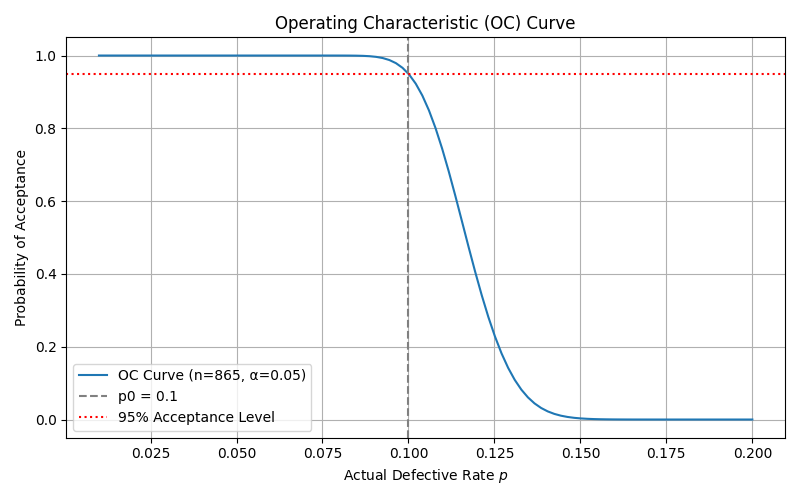
\includegraphics[width=.49\textwidth]{figure/OC_curve_1.png}}
\subcaptionbox{样本空间为609的OC曲线\label{fig:双图b}}
{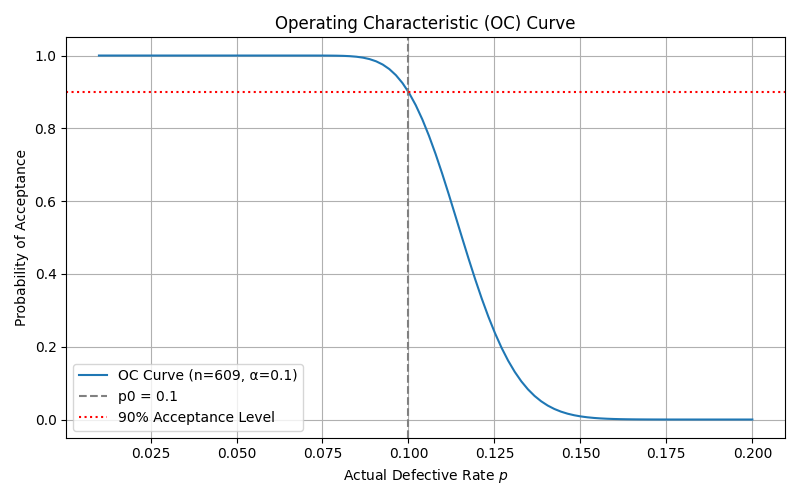
\includegraphics[width=.49\textwidth]{figure/OC_curve_2.png}}
\caption{双图}\label{fig:双图}
\end{figure} 

利用OC曲线可以直观地观察在不同实际不合格率下当前抽样计划的接受概率。从图\ref{fig:双图a}中不难发现,当实际不合格率接近标称值$p_0=0.10$时,接受概率约为95\%,与设定置信水平一致;特别地,我们注意到,随着实际不合格率上升,接受概率陡然下降,说明该检验方案对不合格产品的敏感性较高,即对不合格产品的识别能力较强。

同时,对于质量较好的批次,该方案也能保持较高的接受概率,体现了良好的灵敏度和平衡性。我们从图\ref{fig:双图b}也能得到类似的结论。

此外,根据OC曲线我们还能得出,该种抽样方案下对不合格品的最大容忍数$n_{\text{max}}$,即若发现样本容量中不合格数大于该数值,则拒收,其算式为
\begin{equation}
   n_{\text{max}}=\frac{Z_{\alpha/2}^2p_0(1-p_0)}{d^2}
\end{equation}

对于情形一而言,$n_{\text{max}}=103$,即若抽样容量中不合格数大于103,则拒收。对于情形二而言,$n_{\text{max}}=74$,即若抽样容量大于74,则拒收。

%%%%%%%%%%%%%%%%%%%%%%%%%%%%%%%%%%%%%%%%%%%%%%%%%%%%%%%%%%%%% 
\section{问题二的模型的建立和求解}
\subsection{模型建立}




%%%%%%%%%%%%%%%%%%%%%%%%%%%%%%%%%%%%%%%%%%%%%%%%%%%%%%%%%%%%% 

\section{模型的评价}

\subsection{模型的优点}
\begin{itemize}[itemindent=2em]
\item 优点1:经验样本容量公式计算简便,无需复杂统计工具,并且很好的控制了两类错误,即生产方风险和使用方风险。在信度要求变化时,公式能灵活调整抽样方案,实现了动态调整。

\item 优点2:0-1规划整合复杂逻辑约束,简要精准的描述了“是否”类二元决策问题,简化了模型,适用于多阶段决策。

\item 优点3:

\end{itemize}

\subsection{模型的缺点}
\begin{itemize}[itemindent=2em]
\item 缺点1:问题一假设样本中的次品出现是独立且概率恒定的,但实际生产中,次品可能集中在某些批次,此时抽样结果会低估真实风险。

\item 缺点2:0-1规划的计算复杂度高,变量增多时求解时间指数级增长,增大计算难度。

\item 缺点3:
\end{itemize}
%%%%%%%%%%%%%%%%%%%%%%%%%%%%%%%%%%%%%%%%%%%%%%%%%%%%%%%%%%%%%

\section{模型的改进与推广}

\subsection{改进}
\begin{itemize}[itemindent=2em]
   \item 改进1:问题一可进行成本整合优化:将公式嵌入决策树或线性规划,同时优化样本量、检测成本、拆解费用等。
   \item 改进2:
\end{itemize}


\subsection{推广}
\begin{itemize}[itemindent=2em]
    \item 推广1:经验样本容量公式可推广到供应商来料检验、电子产品可靠性测试与寿命评估、市场质量反馈与售后分析等实际问题。
   \item 推广2:0-1规划可推广到投资组合优化、电路设计、广告投放、网络与路径优化等所有二元决策类问题。
\end{itemize}
\newpage
%%%%%%%%%%%%%%%%%%%%%%%%%%%%%%%%%%%%%%%%%%%%%%%%%%%%%%%%%%%%%
%% 参考文献
\nocite{*}
\bibliographystyle{gbt7714-numerical}  % 引用格式
\bibliography{ref.bib}  % bib源

\newpage
%%%%%%%%%%%%%%%%%%%%%%%%%%%%%%%%%%%%%%%%%%%%%%%%%%%%%%%%%%%%%
%% 附录
\begin{appendices}
\section{文件列表}
\begin{table}[H]
\centering
\begin{tabularx}{\textwidth}{LL}
\toprule
文件名   & 功能描述 \\
\midrule
 exercise\_1.py & 问题一程序代码 \\
 exercise\_2.py & 问题二程序代码 \\
 exercise\_3.py & 问题三程序代码 \\

\bottomrule
\end{tabularx}
\label{tab:文件列表}
\end{table}

\section{代码}
\noindent 
 exercise\_1.py
\lstinputlisting[language=python]{code/exercise_1.py}
exercise\_2.py
\lstinputlisting[language=python]{code/exercise_2.py}
exercise\_3.py
 \lstinputlisting[language=python]{code/exercise_3.py}


\end{appendices}
\end{document}


%%%%%双图模板%%%%%%
% \begin{figure}
% \centering
% \subcaptionbox{炉温曲线示意图\label{fig:双图a}}
% {\includegraphics[width=.4\textwidth]{炉温曲线示意图.png}}
% \subcaptionbox{问题1炉温曲线\label{fig:双图b}}
% {\includegraphics[width=.4\textwidth]{问题1炉温曲线.png}}
% \caption{双图}\label{fig:双图}
% \end{figure} 
%%%%%双图模板%%%%%%